\documentclass[journal]{IEEEtran}

\usepackage{amsmath,amssymb}
\usepackage{graphicx}
\usepackage{booktabs}
\usepackage{cite}
\usepackage{url}

\title{A Non-Archimedean Tree-Scan Diagnostic for Hierarchical Categorical Event Streams}

\author{Abishek Rao M.%
\thanks{The implementation, frozen protocols, claim tables, and artifact manifest accompany this manuscript.}}

\begin{document}
\maketitle

\begin{abstract}
Categorical event streams often contain a domain hierarchy, but flat scan statistics discard shared coarse structure. We encode an ordered categorical tuple as a $p$-adic integer and scan its prefix balls with one-sided binomial log-likelihood ratios. A parent-conditional variant tests child concentration after accounting for observed parent mass. We establish two operational properties: invariance to value relabeling that preserves the hierarchy and a branch-local power advantage over exact-tuple scans when a shift is dispersed across descendants. We then subject the operator to fail-closed temporal tests on 1.53 million real records from IEEE-CIS and two CSE-CIC-IDS2018 days. The conditional scan improves on the unconditional scan on all three datasets, but it does not establish superiority over simple controls: proposed-minus-best-control AUPRC differences are $0.0118$, $-0.0159$, and $-0.0338$, and every paired 95\% bootstrap interval contains zero. The result is therefore a diagnostic contribution, not a detector-superiority claim. The negative controls identify its empirical boundary: hierarchy-specific concentration is detectable, whereas broad diversity or traffic-volume shifts favor entropy or count statistics.
\end{abstract}

\begin{IEEEkeywords}
Anomaly detection, categorical streams, non-Archimedean signal processing, $p$-adic encoding, scan statistics.
\end{IEEEkeywords}

\section{Introduction}
Event streams in fraud and network surveillance mix categorical fields at several resolutions. A transaction may be grouped first by device and card family and then by product and domain; a flow may be grouped by protocol, port band, exact port, and flags. Flat tuples preserve exact combinations but not their shared ancestry. Conversely, marginal statistics erase interactions.

Scan statistics detect localized distribution changes \cite{neill2012fastsubset,rodner2016maxdiv}; changepoint methods provide related temporal formulations \cite{adams2007bocpd,laby2016mixedcusum}. Ultrametric and $p$-adic models represent nested structure directly \cite{ultrametriccommittee2012,khrennikov2023padicdbn}. This letter connects these ideas through an auditable prefix-ball scan for categorical streams. Its contributions are: 1) unconditional and parent-conditional $p$-adic tree scans; 2) analytical statements describing their invariance and branch-local regime; and 3) a frozen, source-backed evaluation designed to fail closed under flat, marginal, hierarchy-order, entropy, and count controls.

The experiments deliberately report a negative cross-dataset gate. This is scientifically useful: it separates an interpretable hierarchy-sensitive statistic from an unsupported claim of predictive superiority.

\section{Tree-Scan Operator}
\subsection{Encoding and Prefix Balls}
Let $x_t=(c_{t1},\ldots,c_{td})$ be an ordered categorical event. Train-only maps assign each category a digit $a_j(c_{tj})\in\{0,\ldots,p-1\}$, where prime $p$ exceeds every field cardinality including an unknown bucket. Define
\begin{equation}
 z_t=\sum_{j=1}^{d} a_j(c_{tj})p^{j-1}.
\end{equation}
The depth-$k$ prefix node is $v_k(z)=z\bmod p^k$. Equality of $v_k$ is membership in the same radius-$p^{-k}$ $p$-adic ball. Thus early tuple fields are coarse digits and later fields refine the branch.

Only normal training rows estimate node probabilities. With additive smoothing $\alpha$, a depth-$k$ node $v$ has probability $\hat p_{kv}$. Held-out events are time ordered and divided into $B$ equal-count blocks. For block $b$ of size $n_b$, let $N_{bkv}$ be the number of events in node $(k,v)$. The one-sided excess statistic is
\begin{equation}
 \ell(N,n,p)=
 \begin{cases}
 nD_{\mathrm{KL}}(N/n\Vert p),&N>np,\\
 0,&\text{otherwise},
 \end{cases}
\end{equation}
where $D_{\mathrm{KL}}$ is Bernoulli divergence. The unconditional score is $S_b=\max_{k,v}\ell(N_{bkv},n_b,\hat p_{kv})$.

\subsection{Parent-Conditional Residual}
High-level volume changes can make many descendants appear excessive. For $k>1$, let $\pi(v)$ be the parent node, $N_{b,k-1,\pi(v)}$ its observed block count, and $\hat p_{v\mid\pi(v)}$ the train-normal child probability. We score
\begin{equation}
 S_b^{\mathrm{cond}}=\max_{k>1,v}\ell\!\left(N_{bkv},N_{b,k-1,\pi(v)},\hat p_{v\mid\pi(v)}\right).
\end{equation}
This asks whether a child receives excess mass conditional on the parent mass actually present in the block.

\subsection{Operational Properties}
\textit{Proposition 1 (hierarchy-preserving relabeling).} If each field's category symbols are permuted while its digit map is permuted identically, node memberships, counts, and both scan scores are unchanged.

\textit{Justification.} The operator depends on prefix equality, not numeric digit magnitude. A bijection merely renames nodes at each depth.

\textit{Proposition 2 (branch-local aggregation).} Suppose an anomalous block increases a prefix probability from $q$ to $q+\delta$. Its expected excess score is
\begin{equation}
 nD_{\mathrm{KL}}(q+\delta\Vert q)
 \approx \frac{n\delta^2}{2q(1-q)}.
\end{equation}
If this shift is divided equally among $M$ exact descendant tuples, the strongest exact-tuple score is approximately reduced by $M^2$ under comparable baselines. Prefix aggregation is therefore beneficial only when affected tuples share a meaningful branch. Broad diversity changes need not satisfy this condition and can favor entropy controls.

\section{Fail-Closed Evaluation}
\subsection{Datasets and Frozen Protocol}
IEEE-CIS fraud detection \cite{ieeecis2019} contains 590,540 transactions. CSE-CIC-IDS2018 \cite{sharafaldin2018ids} contributes 331,100 Thursday and 613,071 Wednesday flows. Each dataset is temporally sorted, split 70/30, and the held-out portion is divided into 96 blocks. A block is positive under the frozen upper-quartile block event-rate rule. Labels filter normal training rows and evaluate blocks; they never enter a hierarchy.

The IEEE hierarchy orders DeviceType, card6, card4, ProductCD, and P\_emaildomain. The CSE hierarchy orders protocol, port band, destination port, and SYN, ACK, and PSH flag counts. Wednesday was preregistered before download or label inspection and reused the Thursday hierarchy and parameters unchanged.

Mandatory controls are exact-tuple scan, marginal-column scan, reversed hierarchy, five fixed random hierarchies, temporal category entropy, and transaction count. The primary metric is block AUPRC. Uncertainty is a paired 500-resample block bootstrap of best proposed minus best control AUPRC. A gate passes only when the proposed method beats every control, the 95\% interval is strictly positive, and $\Pr(\Delta\leq0)\leq0.05$.

\subsection{Results}
\begin{table}[t]
\caption{Frozen block-surveillance gates. CI is paired 95\% bootstrap interval for proposed minus best control AUPRC.}
\label{tab:gates}
\centering
\footnotesize
\setlength{\tabcolsep}{3.2pt}
\begin{tabular}{lcccc}
\toprule
Dataset & Proposed & Control & $\Delta$ & 95\% CI \\
\midrule
IEEE-CIS & .2977 & .2860 & +.0118 & [-.0705,.1222] \\
CSE Thu. & .5242 & .5401 & -.0159 & [-.1860,.1564] \\
CSE Wed. & .2153 & .2491 & -.0338 & [-.1416,.0396] \\
\bottomrule
\end{tabular}
\end{table}

The conditional score exceeded the unconditional score by 0.1070, 0.0145, and 0.0193 AUPRC on IEEE-CIS, Thursday, and Wednesday, respectively. Table~\ref{tab:gates} and Fig.~\ref{fig:gates} show the stricter comparison. IEEE-CIS has a small positive point difference over transaction count, but its interval crosses zero and $\Pr(\Delta\leq0)=0.33$. Entropy is the strongest control on both CSE days; differences are negative with probabilities 0.506 and 0.820. All three gates therefore return the frozen status \texttt{diagnostic\_only\_failed\_q1\_tree\_scan\_gate}.

\begin{figure}[t]
\centering
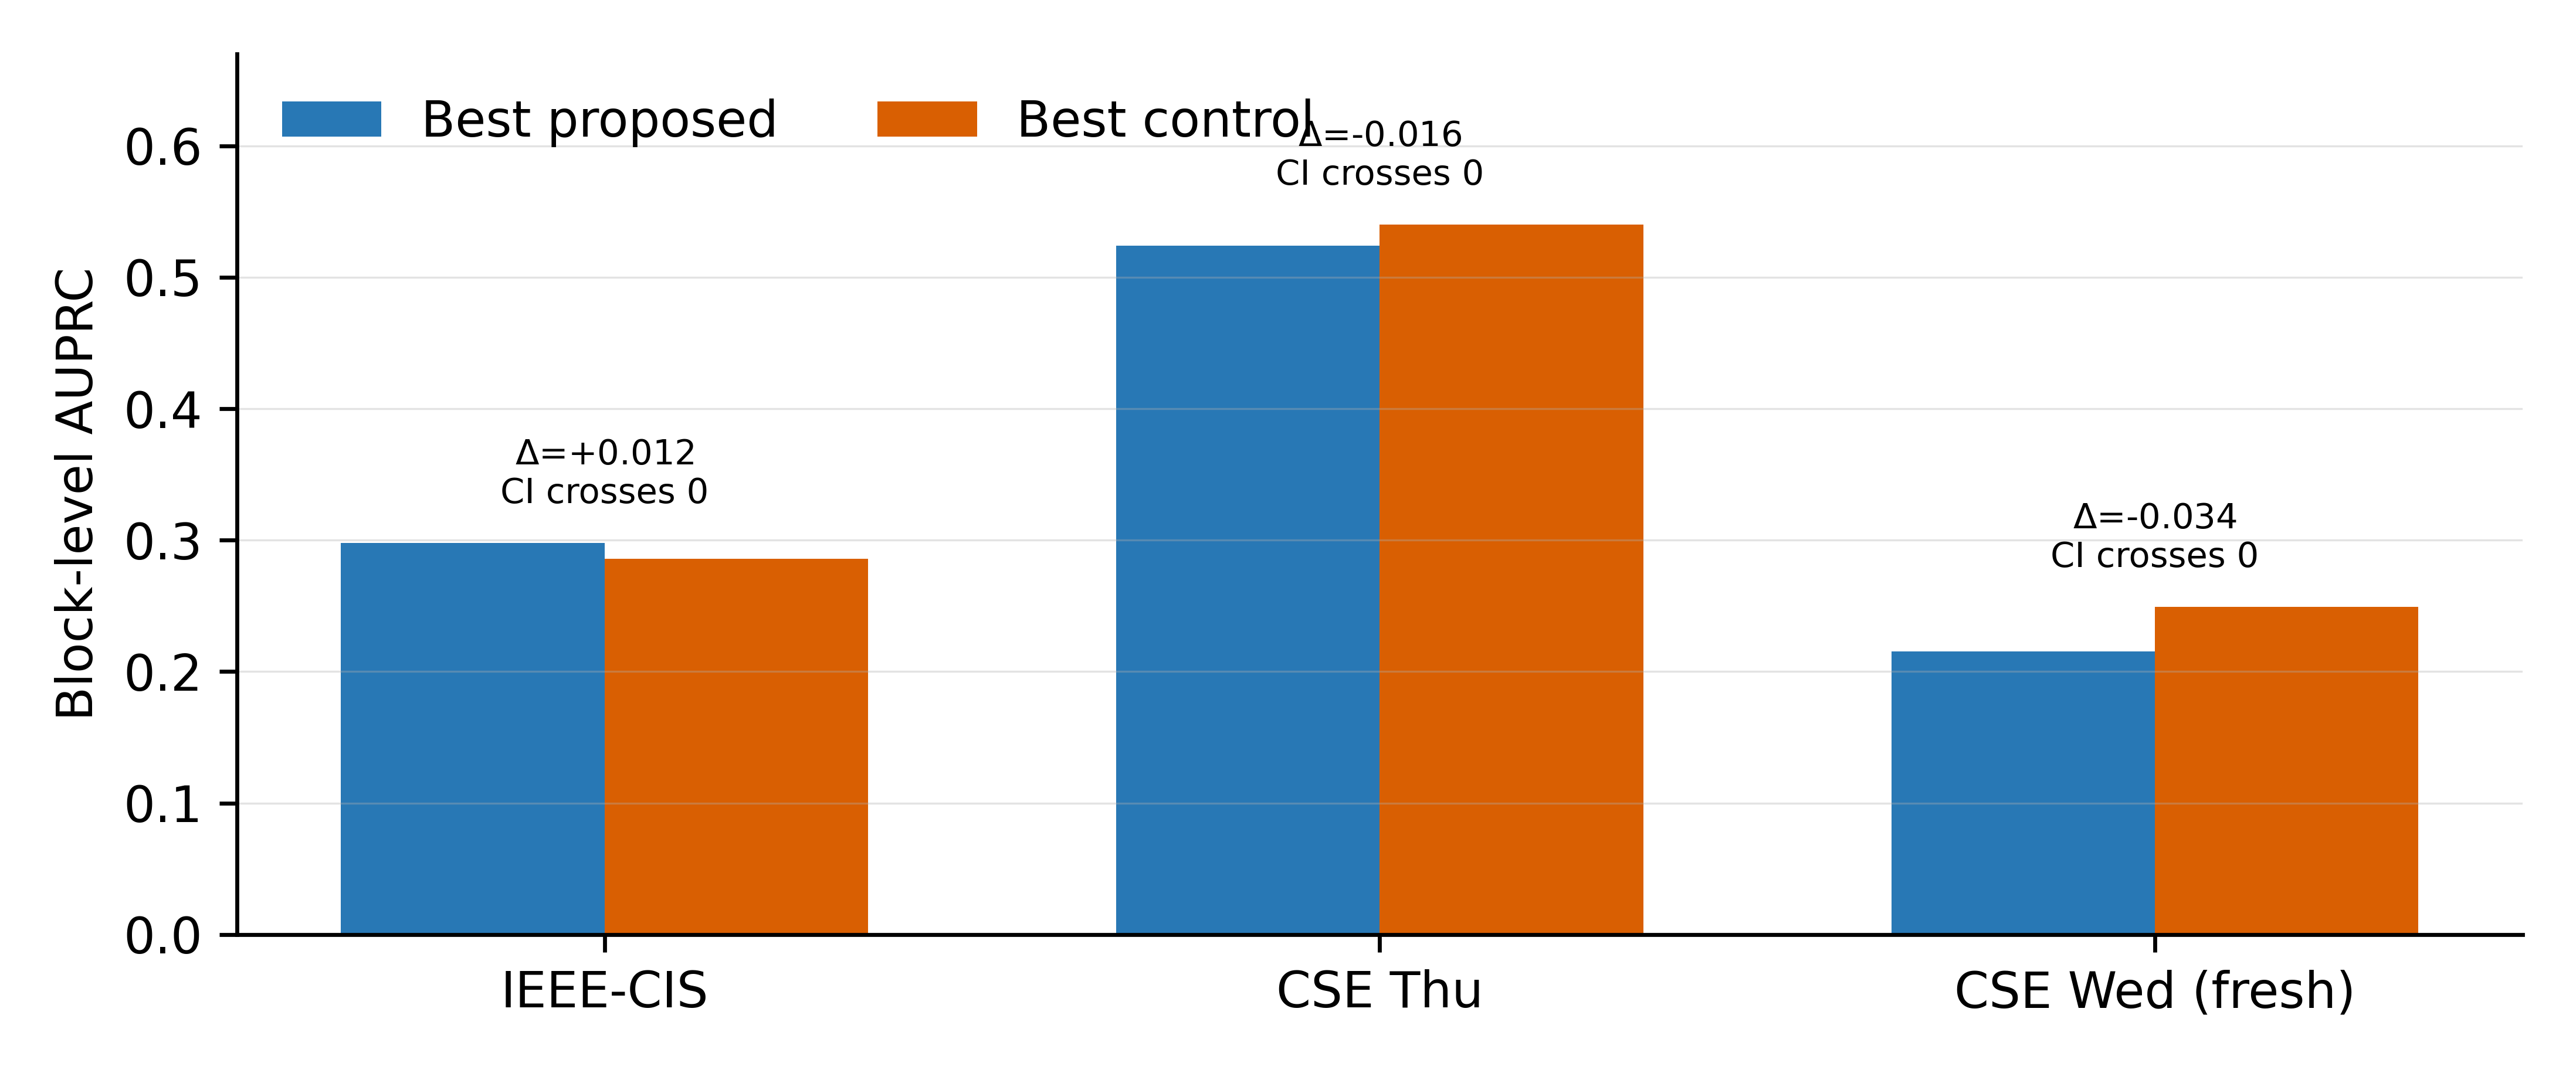
\includegraphics[width=\columnwidth]{tree_scan_artifacts/cross_dataset_gate_auprc.png}
\caption{Best proposed and best control block AUPRC. No paired interval excludes zero. Wednesday is a fresh preregistered validation.}
\label{fig:gates}
\end{figure}

The two CSE failures are informative rather than contradictory. Parent conditioning consistently removes some coarse traffic-volume effect, but category entropy still wins when attacks alter broad compositional diversity rather than concentrating mass in one semantic branch. The result matches Proposition 2's boundary condition. It also shows why a flat or weak control set would overstate the method.

\section{Discussion and Conclusion}
The proposed operator supplies a transparent localization output: block, depth, prefix node, observed count, expected count, and LLR. It is computationally practical because prefix counts are accumulated once per depth and block. Exact-output regression tests verify that this optimization leaves every claim-table value unchanged.

The study has important limits. Hierarchies are domain choices, block labels are derived from event-rate quartiles, and 96 blocks make uncertainty substantial. IEEE-CIS is a fraud benchmark while CSE-CIC is network intrusion data, so the external tests probe operator behavior rather than task-identical transfer. Most importantly, no dataset meets the preregistered superiority gate.

We conclude that parent-conditional non-Archimedean scanning is an interpretable diagnostic for branch-local categorical concentration. Current evidence does not support calling it a superior fraud or intrusion detector. A stronger empirical claim requires a new independently preregistered dataset, prospective hierarchy specification, and positive controlled intervals; tuning on the failed held-out days would invalidate that claim.

\bibliographystyle{IEEEtran}
\bibliography{references}

\end{document}
